\usepackage[authoryear,round]{natbib}
\usepackage{multirow}

\newcommand{\sheetnum}{%
	11
}
%\setcounter{section}{\sheetnum-3}
\newcommand{\tutorialtitle}{%
    Density Estimation and Estimation bias
}
\newcommand{\tutorialtitleshort}{%
	Density Estimation
}
% for slides
\subtitle{\sheetnum \tutorialtitle}

\maxdeadcycles=1000 % Workaround for ! Output loop---100 consecutive dead cycles because of too many figures

% The following use of algroithms does not work well with the notes:
%
%
%
%
% instead use the following for your algorithms:
%
%\begin{figure}[!t]
%\removelatexerror
%\begin{algorithm}[H]
    % your algo here
    %\label{alg:algolabel}
    %\caption{algocaption}
%\end{algorithm}
%\end{figure}
%\begin{algorithm}
% Below is the definition for the command \removelatexerror:
\makeatletter
\newcommand{\removelatexerror}{\let\@latex@error\@gobble}
\makeatother

\begin{document} %%%%%%%%%%%%%%%%%%%%%%%%%%%%%%%%%%%%%%%%%%%%%%%%%%%%%%%

\sheet{\sheetnum}{\tutorialtitleshort}

\ttopic{\tutorialtitle}

\columnratio{0.2,0.8}\textbf{}
\begin{paracol}{2}
%\setlength{\columnseprule}{0.1pt}
%\setlength{\columnsep}{5em}

\begin{rightcolumn}

% notes version will ignore it
\begin{frame}
\titlepage
\end{frame}

\setcounter{tocdepth}{2}
\begin{frame}
\mode<presentation>{
\tableofcontents[subsubsectionstyle=show/show/show/hide]
}
\mode<article>{
\tableofcontents
}
\end{frame}

\newpage

\mode<all>
\section{Density Estimation}


\mode<presentation>{
\begin{frame} 
    \begin{center} \huge
        \secname
    \end{center}
    %\begin{center} \large
        %\subsecname
    %\end{center}
	
\end{frame}
}

\subsection{What and Why?}

\begin{frame}{\secname:~\subsecname}

\notesonly{
We observe data. 
This data is generated by some unknown probability distribution. Each observation is a sample from this distribution.
When we talk about density estimation, we are talking about recovering the underlying probability density function that produced the observed samples.
}

\question{Why do we care about estimating densities? What can we do with an estimated density?}

\begin{itemize}
\item data exploration
\item visualization for 1D and 2D data (no dimensionality reduction)
\item deduce moments (mean, variance, \ldots)
\item describe the data in compact form (e.g. ``this data follows a Gaussian with mean $\mu$ and variance $\sigma^2$'')
\item generate new data
\item unsupervised anomaly detection
\end{itemize}

\end{frame}

\subsection{Strategies}

\begin{frame}{\subsecname}

2 strategies:

\begin{enumerate}[(A)]
\item \textbf{parametric} methods:
\\ We assume that the data follows some class of distribution and we estimate its paramters (e.g. fit a Gaussian around this data)
\item \textbf{non-parametric}\footnote{non-parametric does not means it is void of paramters. 
It is just that the parameters do not directly correspond to the classical parameters of densities such as mean and variance.} methods: 
data-driven. Estimate the density with as few assumptions as possible (e.g. Kernel\footnote{Not tied to Mercer Kernels like in Kernel PCA. A kernel is just some non-negative function.} density estimation)
\end{enumerate}

\end{frame}

\begin{frame}
\only<1>{\frametitle{Histograms}}
\only<2>{\frametitle{Normalized Histograms $\rightarrow$ density}}

\notesonly{
Many people habe already encountered density estimation in the form of histograms.
}

\begin{minipage}{0.48\textwidth}
\begin{center}
	\includegraphics<1->[width=0.95\textwidth]{./img/hist}
	\notesonly{\captionof{figure}{Example histogram}}
\end{center}
\end{minipage}
\begin{minipage}{0.48\textwidth}
\begin{center}
	\includegraphics<2>[width=0.95\textwidth]{./img/hist_density}
	\notesonly{\captionof{figure}{Example density using a normalized histogram}}
\end{center}
\end{minipage}

\end{frame}

\subsection{Kernel density estimation (KDE)}

\mode<presentation>{
\begin{frame} 
    \begin{center} \huge
        \subsecname
    \end{center}
    \begin{center}
        Data-driven ``histogram bin placement''
    \end{center}
	
\end{frame}
}

\begin{frame}{\subsecname}
	
\begin{center}
	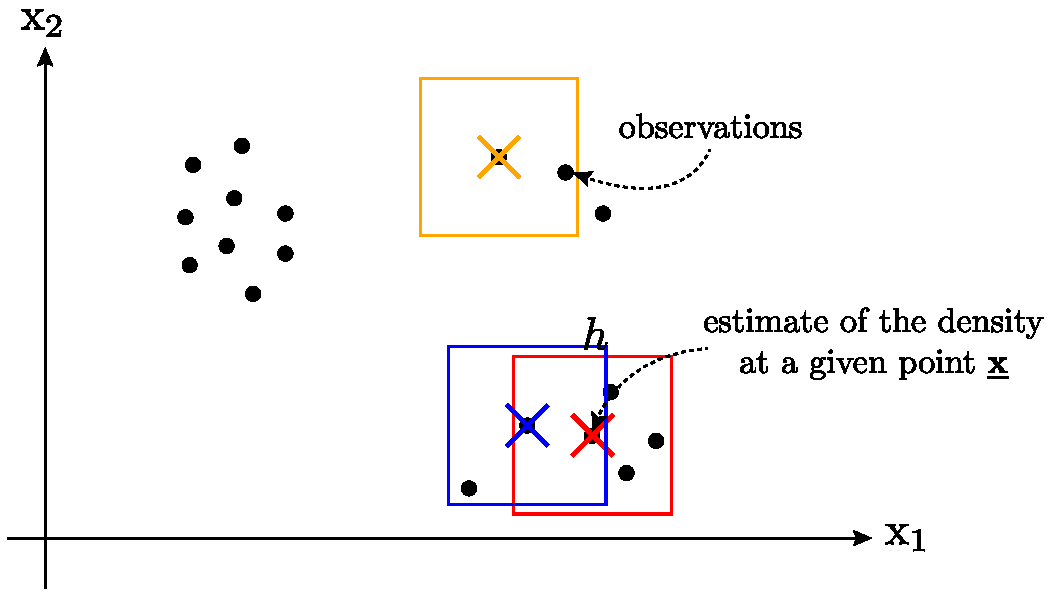
\includegraphics[width=0.6\textwidth]{./img/section1_fig1}
	\notesonly{\captionof{figure}{Kernel density estimation}}
\end{center}

Count the number of data points within a volume $V$ centered on $\vec{x}$.
Normalize to turn into a density estimate $\widehat{P}(\vec{x})$.

\end{frame}

\begin{frame}[t]{``Gliding histograms'' -- 1D case}
\small
\vspace{-0.3cm}
\slidesonly{Count the number of data points within a volume $V$ centered on $\vec{x}$.\\\vspace{0.1cm}}
Histogram kernel:
\begin{equation*}
\begin{array}{ll}
H({u}) = \left \{ \begin{array}{ll}
1, & u \in (-\frac{1}{2}, \frac{1}{2}) \\\\
0, & \text{else}
\end{array} \right.
\end{array}
\end{equation*}
Density estimate (``gliding histogram''):
\vspace{-0.3cm}
\begin{equation*}
	\widehat{P}({x};h) = 
	 \kern-3ex \underbrace{ \frac{1}{h}}_{
	\substack{ \text{normalization}}}
	 \kern-1.5ex 
\cdot \underbrace{ \frac{1}{p} 
	\overbrace{ \sum\limits_{\alpha = 1}^p
		H \bigg( \frac{{x} - {x}^{(\alpha)}}{
			h} \bigg) }^{
		\substack{\text{number of data points}\\
			\text{within window } (x-\frac{1}{2}, x+\frac{1}{2}) \\
			\text{ around } {x}}} }_{
	\text{fraction of data points}}
\end{equation*}
Histogram kernels lead to discontinuous pdf estimates $\leadsto$ use other kernels for smooth pdf estimates. 
\end{frame}


\begin{frame}[t]{``Gliding histograms'' -- N-dim data}
\small
Let $\vec x \in \R^N$:\\
%\vspace{-0.3cm}
\slidesonly{Count the number of data points within a volume $V$ centered on $\vec{x}$.\\\vspace{0.1cm}}
Histogram kernel:
\begin{equation*}
\begin{array}{ll}
H(\vec{u}) = \left \{ \begin{array}{ll}
1, & |u_j| < \frac{1}{2}, \forall j \in 1, \ldots, N \\\\
0, & \text{else}
\end{array} \right.
\end{array}
\end{equation*}
Density estimate (``gliding histogram''):
\vspace{-0.3cm}
\begin{equation*}
	\widehat{P}(\vec{x}) = \kern-3ex \underbrace{ \frac{1}{h^N} }_{
	\substack{ \text{normalization} \\
		\text{(``density''!)}}}
		\kern-1ex
\cdot \underbrace{ \frac{1}{p} 
	\overbrace{ \sum\limits_{\alpha = 1}^p
		H \bigg( \frac{\vec{x} - \vec{x}^{(\alpha)}}{
			h} \bigg) }^{
		\substack{\text{number of data points}\\
			\text{within volume } V 
			\text{ around } \vec{x}}} }_{
	\text{fraction of data points}}
\end{equation*}
Histogram kernels lead to discontinuous pdf estimates $\leadsto$ use other kernels for smooth pdf estimates. 
\end{frame}

\begin{frame}{Kernels}

\begin{center}	
	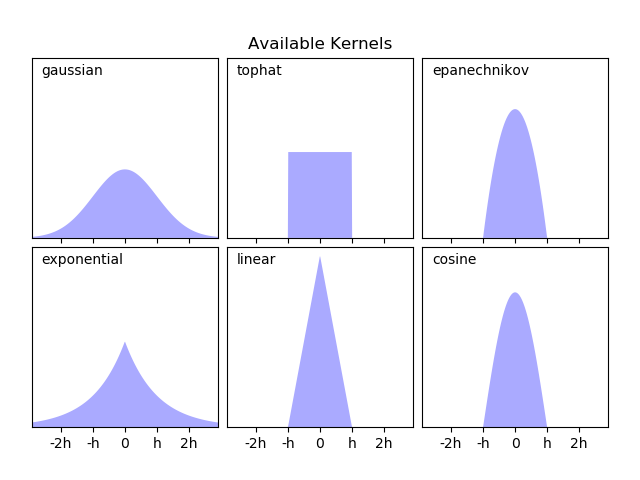
\includegraphics[width=0.6\textwidth]{./img/sphx_glr_plot_kde_1d_0021}
	\notesonly{\captionof{figure}{Kernel functions}}
\end{center}

{\footnotesize
Figure from https://scikit-learn.org/stable/modules/density.html
}


\end{frame}

\begin{frame}{Histogram vs. KDE}

\svspace{-3mm}

\begin{center}	
	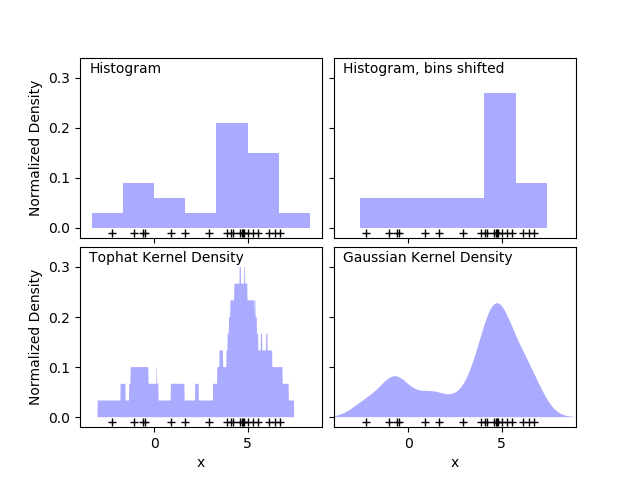
\includegraphics[width=0.5\textwidth]{./img/sphx_glr_plot_kde_1d_0011}
	\notesonly{\captionof{figure}{Histograms vs. KDE using different kernel functions}}
\end{center}

\svspace{-3mm}

Gaussian Kernel (1D case):

\svspace{-3mm}

\begin{equation}
H(u) = \frac{1}{\sqrt{2\pi}} \exp\Big({\frac{-u^2}{2}}\Big)
\end{equation}

\begin{equation}
\widehat{P}({x}, h) = \frac{1}{h p \sqrt{2\pi}} \sum_{\alpha=1}^p \exp \Big\{ -\frac{(x-x^{(\alpha)})^2}{2h^2} \Big\}
\end{equation}

{\footnotesize
Figure from https://scikit-learn.org/stable/modules/density.html
}

\end{frame}

\subsubsection{Choice of kernel width}


\begin{frame}{\subsubsecname}

\begin{figure}
	\centering
	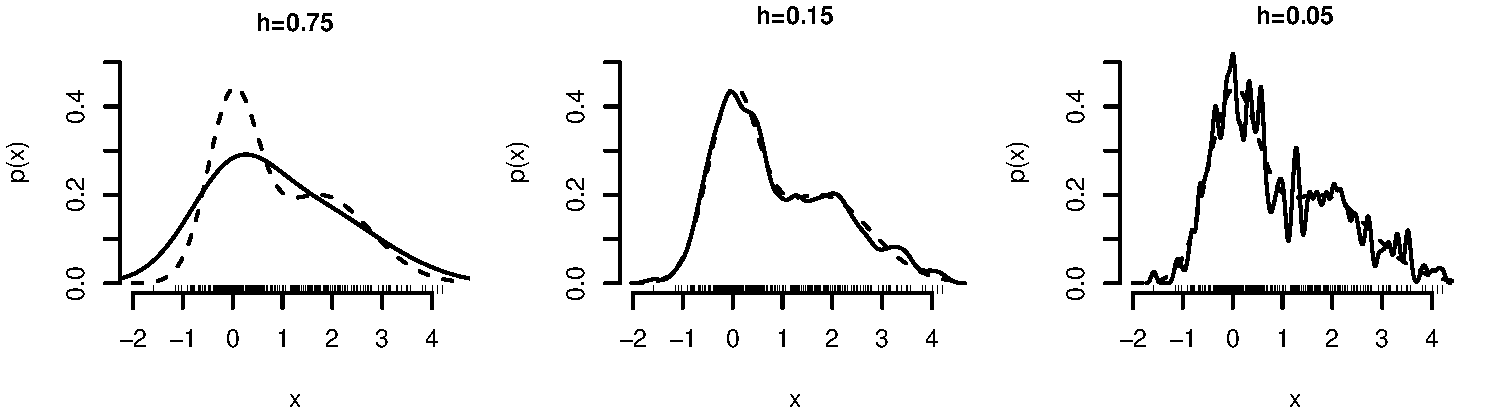
\includegraphics[width=\textwidth]{img/densExamples.pdf}\
	\notesonly{\captionof{figure}{Effect of kernel width h}}
\end{figure}

Choice of kernel width $h > 0$ $\Rightarrow$ model selection / validation


\end{frame}

\mode*

\clearpage

\mode<all>
\subsection{Maximum Likleihood Estimation (MLE)}

\mode<presentation>{
\begin{frame} 
    \begin{center} \huge
        \subsecname
    \end{center}
    \begin{center}
        Finding a model that explains the data
    \end{center}
	
\end{frame}
}

\begin{frame}{What does maximizing the likelihood mean?}

A crude way of understanding maximum likelihood estimation:\\

A density estimate that maximizes the likelihood will

\begin{itemize}
\item yield non-zero probability for samples that resemble the observed data
\item yield higher probability for samples that occur more frequently in the observed data
\end{itemize}

\end{frame}

\begin{frame}{The likelihood function}

 \begin{block}{generative model}
    \begin{equation}
        \begin{array}{lr}
        \widehat{P}(\vec{x};\vec{w}) 
        & \substack{ \text{probability density for the} \\
                   \text{generation of one data point} }
        \end{array}
\end{equation}
  \end{block}
%\pause 
\vspace{4mm}

\begin{block}{likelihood of the model = p(observations given the model)}
 assuming iid. observations:
\begin{equation}
                \widehat{P}\big( \big\{ \vec{x}^{(\alpha)} \big\};\vec{w} \big)
                = \prod\limits_{\alpha = 1}^p \widehat{P}\big(\vec{x}^{(\alpha)}
                        ;\vec{w} \big)
\end{equation}
\end{block}

\end{frame}

\subsection{Model selection}
\begin{frame} \frametitle{Model selection and Maximum Likelihood}
\begin{equation*}
        \widehat{P}\big(\big\{\vec{x}^{(\alpha)}\big\};\vec{w}\big)
                \eqexcl \max_{\vec{w}}
\end{equation*}
\textbf{intuition:} select the model which generates the observed data with high probability\\
%\pause
\vspace{5mm}
\textbf{in practice:} minimization of the negative $\log$-likelihood
\begin{equation*}
        \begin{array}{ll}
                p \cdot E_{[\vec{w}]}^T
                & = -\ln \widehat{P}\big(\big\{\vec{x}^{(\alpha)}\big\}
                        ;\vec{w}\big) \\\\
                & = -\sum\limits_{\alpha = 1}^p \ln \widehat{P}
                        \big( \vec{x}^{(\alpha)};\vec{w} \big)
                \;\; \eqexcl \;\; \min_{\vec{w}} 
        \end{array}
\end{equation*}
%\pause
Equivalent to:
\begin{equation}
	\dkl\Big[P(\vec{x}),\widehat{P}(\vec{x};\vec{w})\Big] = \int d \vec{x} P(\vec{x}) \ln 
		\frac{P(\vec{x})}{\widehat{P}(\vec{x};\vec{w})} = \min_{(\vec{w})}
\end{equation}

except that $P(\vec{x})$ is unknown.

\end{frame}

\begin{frame}{Generalization on unseen data}

minimal $E^T$ is not as good as we think. We need to validate the likelihood on a test set.

\end{frame}

\mode*

\clearpage

\mode<all>
\subsection{Parametric density estimation}

\mode<presentation>{
\begin{frame} 
    \begin{center} \huge
        \subsecname
    \end{center}
    \begin{center}
        Fitting the parameters of a Gaussian/Laplacian/... to the data
    \end{center}
	
\end{frame}
}

%%%%%%%%%%%%%%%%%%%%%%%%%%%%%%%%%%%%%%%%%%%%%%%%%%%%%%%%%%%%%%%
\begin{frame}[t]{The multivariate Gaussian}
\smaller
\svspace{-0.8cm}
\begin{alignat*}{2}
&\widehat{P}\left(\left\{ \vec{x}^{(\alpha)} \right\}; \vec{\boldsymbol \mu}, \vec{\Sigma} \right) &&= \left( \frac{1}{\sqrt{(2\pi)^N \det \vec{\Sigma}}} \right)^p \cdot \prod_{\alpha=1}^{p} \exp \left(-\frac{1}{2} \left(\vec{x}^{(\alpha)} - \vec{\boldsymbol \mu} \right)^\top \vec{\Sigma}^{-1} \left(\vec{x}^{(\alpha)} - \vec{\boldsymbol \mu} \right) \right) \\[10pt]
&E^T\left( \vec{\boldsymbol \mu}, \vec{\Sigma} \right) &&= - \ln \widehat{P}\left(\left\{ \vec{x}^{(\alpha)} \right\}; \vec{\boldsymbol \mu}, \vec{\Sigma} \right) \\
& &&= \frac{p \cdot N}{2} \ln(2\pi) + \frac{p}{2} \ln(\det \vec{\Sigma}) + \frac{1}{2} \sum_{\alpha=1}^{p} \left(  \vec{x}^{(\alpha)} - \vec{\boldsymbol \mu} \right)^\top \vec{\Sigma}^{-1} \left(  \vec{x}^{(\alpha)} - \vec{\boldsymbol \mu} \right)
\end{alignat*}
\\\vspace{0.2cm}
minimization of $E^T$ (necessary conditions):
\vspace{-0.1cm}
\begin{align*}
\frac{\partial E^T}{\partial \vec{\boldsymbol \mu}} = \vec{0} \quad &\Rightarrow \quad \vec{\boldsymbol \mu}^* = \frac{1}{p} \sum_{\alpha=1}^{p} \vec{x}^{(\alpha)}  &&\text{(empirical average)}\\
\frac{\partial E^T}{\partial \vec{\Sigma}} = \vec{0} \quad &\Rightarrow \quad \vec{\Sigma}^* = \frac{1}{p} \sum_{\alpha=1}^{p} (\vec{x}^{(\alpha)} - \vec{\boldsymbol \mu}^*) (\vec{x}^{(\alpha)} - \vec{\boldsymbol \mu}^*)^\top &&\text{(empirical covariance matrix)}
\end{align*}

remark: $\vec{\boldsymbol \mu}^*$ is unbiased, but $\vec{\Sigma}^*$ is a biased estimator (cf. next section)

\end{frame}

\mode*

\clearpage

\mode<all>
\section{Estimator bias}

\mode<presentation>{
\begin{frame} 
    \begin{center} \huge
        \secname
    \end{center}
    \begin{center}
        How good is our estimation method?
    \end{center}
	
\end{frame}
}

%%%%%%%%%%%%%%%%%%%%%%%%%%%%%%%%%%%%%%%%%%%%%%%%%%%%%%%%%%%%%%%
\begin{frame}{Parameters are also random variables}

Assume $\vec x^{(\alpha)} \sim P(\vec x; \vec w^*)$, i.e. $\vec x^{(\alpha)}$ is a random vector, and $\vec w^*$ the true parameters of a the data generating distribution.\\

\svspace{3mm}

Our estimator yields an estimate $\widehat{\vec w} = f(\vec x^{(1)}, \ldots,\vec x^{(p)})$ $\Rightarrow$ $\widehat{\vec w}$ is also a random variable\\

\svspace{3mm}

Example: MLE $\widehat{\vec w}_{\text{ML}} = \argmax_{\vec w} \widehat P(\vec x^{(1)}, \ldots,\vec x^{(p)}; \vec w)$\\

\pause 

\question{Where does the randomness come from?}

\pause

-Different data sets with $p$ samples from the same distribution lead to different estimates $\widehat{\vec w}$

\pause

\svspace{3mm}

$\Rightarrow$ The random vector $\widehat{\vec w}$ has moments, e.g. mean $\langle \widehat{\vec w} \rangle_{P(\vec x^{(1)}, \ldots,\vec x^{(p)}; \vec w^*)}$

\end{frame}

\subsection{Bias of an estimator}

\begin{frame}{\subsecname}

bias $\vec b := \langle \widehat{\vec w} \rangle - \vec w^*$

If $b=0$, then our estimator is \textbf{un}biased

\underline{Interpretation}: Draw multiple data sets of size $p$, then the estimated parameters will surround the true vector $\vec w^*$.

\begin{center}
	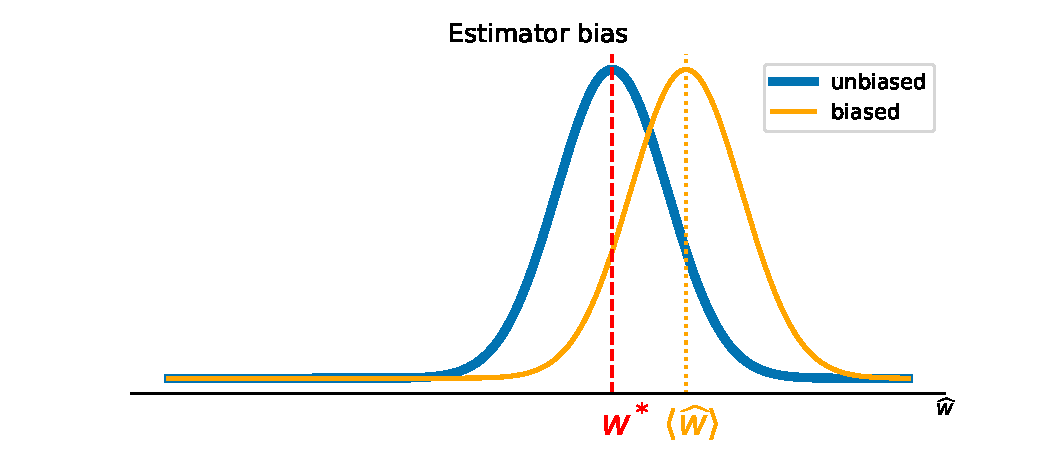
\includegraphics[width=0.6\textwidth]{img/bias.pdf}
	\notesonly{\captionof{figure}{Estimator bias}}
\end{center}


\end{frame}

\subsection{Variance also plays a role}

\begin{frame}{\subsecname}

\begin{center}
	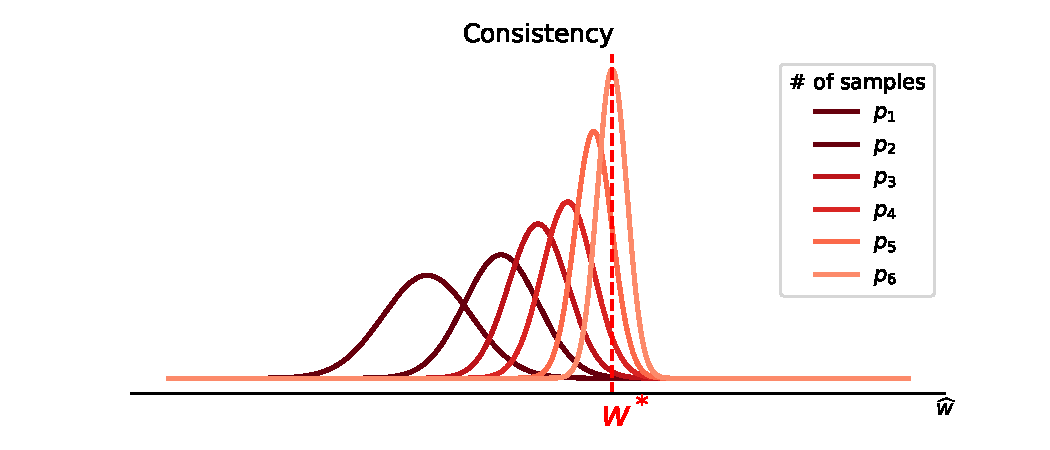
\includegraphics[width=0.6\textwidth]{img/consistency.pdf}
	\notesonly{\captionof{figure}{A consistent estimator converges in probability to the true value when given more data.}}
\end{center}

\end{frame}

\mode*

\clearpage

%\section{References}
%\begin{frame}[allowframebreaks] \frametitle{References}
	%\scriptsize
	%\bibliographystyle{plainnat}
	%\bibliography{bibliography}
%\end{frame}

\end{rightcolumn}
\end{paracol}

\end{document}
